\chapter{Introduction}
\begin{figure}[htb]
	
\includegraphics{../images/sky-690293_1920.jpg}
	\label{fig:sky}
\end{figure}

\justify
The term DevSecOps\index{DevSecOps} is an amalgam of the words
Development, Security, and Operations. The combination of
these three words represents the overlap and interplay between
sometimes disparate work functions. The degree to which these three 
realms overlap depends on the structure of a given organization.
Simply put, DevSecOps lives at the intersection of
application development and/or Infrastructure as Code
development, Information Security, and Network Operations.
\justify
This combined job functionality has some overarching goals, for
example the movement of secure
software through an ongoing series of incremental test and deployment
phases, often referred to as pipelines\index{pipeline}. We will explore this and other
ways our platforms and pipelines
are becoming more abstract from the viewpoint of the tools that we use to do it.
Definition of our infrastructure in reusable software patterns is another big objective
in the DevSecOps paradigm. This Infrastructure as Code (IaC)\index{Infrastructure as Code (IaC)}
is the platform
upon which our application software work products flow through a cycle of Continuous
Deployment or Continuous Delivery (CD)\index{Continuous Delivery (CD)}.
\justify
In recent years, there has been a move away from traditional
"Big Iron" running in privately owned data centers under a
single administrative domain. The shift is towards shared
compute resources. These shared resources have much of the
maintenance requirements and complexity abstracted away.

\justify
The world is changing with respect to how software is created and maintained.
Folks at the leading edge in today's computing industry are not just building
software, but are curating it through a cyclical process of continuous development,
testing, use, and improvement. With increasing frequency, applications and
workloads are moving to computing environments that are abstracted away, managed
by invisible armies of engineers at companies other than their own. Of course
we are referring to those multitenant cloud type computing landscapes. Passing
one or more fully encapsulated applications to a cloud provider for the purposes
of having "someone else" host it as a production environment has become
commonplace. Further, cloud service providers are adding new features and capabilities
at breakneck speed.

\begin{figure}[!htb]
	\centering
	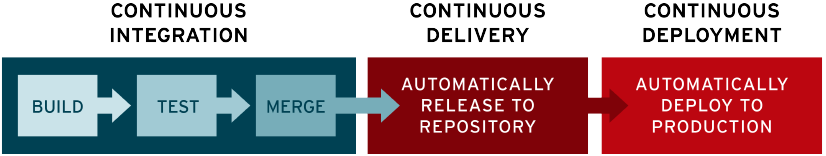
\includegraphics[scale=0.35]{../images/ci-cd-flow-desktop_0.png}
	\caption{Typical pipeline stages.}
	\label{fig:stages}
\end{figure}

\justify
To the extent possible, the modern software project team aligns around an
attempt to realize gains in performance of our people and projects by
leveraging automation and Agile development practices throughout the
feature development cycle.

\justify
At the time of this writing in 2020, about 40\% of production workloads are
running on containers or are deployed in low cost serverless configurations.
Bare metal and virtual machines currently host a bit over 60\% of production
workloads. Containerized workload use is expected to increase even more in
the coming years. Conversely, bare metal and VM usage is expected to
decrease in the coming years.

\justify
It's not a question of if, but how quickly commoditization of compute resources
will replace private corporate data centers, perhaps resulting in only a
few main providers of cloud computing resources. This shift has been likened
to how power generation and distribution became centralized
in the previous century, now the domain of a few large utility companies.
Nothing beyond considerations of time, money, and practicality stop you
from making your own electricity, but most folks are keen to invest their
efforts in other pursuits.

\justify
Strategic decisions are about defining the direction of a team and overseeing
the allocation of the resources needed to pursue the goals of the entire
business organization. These are the sorts of things the upper managers are
thinking about. The linking of the strategic direction to tactical tasks is
done with operational planning. This managerial view might be best framed in
year-long increments. Think of operational planning as the purview of line
and middle managers who detail the goals and milestones, and capture metrics
on progress toward strategic goals of the business. Finally, tactical concerns
are the short range objectives of a team within a department or business unit.
The tactical viewpoint tends to span a time period of one year or less and is
the domain of the individual contributor and technical champion. This is the
"fun stuff", where you get to be closest to the code. This book will focus
on the practical, by and for those who want to be tactical. There is also
an interdependence on the logistical here. Logistics in our context refers to
the things that make it possible for the tactical to succeed, and look good
while doing it!

\justify
Among the tactical practitioners, we can further decompose responsibility into
varying degrees of Development, Security, and Operational work. The typical
person in a developer type role
is often working under stringent deadlines to "ship code", which means their
main focus is "getting code out the door" to keep management happy. The person
working in the security role is mostly concerned with prevention of the abuse
of the technology assets of a business.

\justify
In this book, we will explore a combination of techniques that can refresh your
skills and align your projects with the technological leading edge. We will
introduce various popular technologies, then use common bits and pieces of
these to create a secure build pipeline for our lab and development work,
test, and even production environments. The techniques here are meant to help
the security-minded developer sharpen her or his skills, and introduce tips
and tactics that benefit the teams they are a part of. There are many, many
ways to reach similar goals these days with the preponderance of Open Source
and commercial tools that are available. By focusing on a few we can blaze a
trail to success in our projects.

\justify
We have a goal in mind of selecting complementary tools and process to construct
and streamline our ways of working. We will attempt to leverage these ways to
get us quickly and securely to a working example lab environment. Along the
way we should strive for simplicity and reduction of complexity when possible.
Experience tells us that tools, security measures, and process that are too cumbersome
or otherwise prohibitive in nature are typically circumvented, or even abandoned.
Complexity in our processes become the snags and side projects that are the
enemy of productivity.

\justify
Refuse to shave more yaks than absolutely necessary!
